\section{Parabolic p-Laplace Problem on an L-shaped Domain}
\label{sec:lshape-plaplace}

The preceding numerical settings were smooth. They were useful for verifying the automated residual localisation, but they did not provide a comparison between goal-oriented and uniform refinement. The final experiment therefore considers a parabolic $p$-Laplace problem on an L-shaped domain. The re-entrant corner introduces the classical $r^{2/3}$ singular mode, while a spatially and temporally localised nonlinear functional tests whether the adaptive method concentrates resolution only where it is relevant to the prescribed quantity of interest, despite the reduced spatial regularity at the re-entrant corner.

The experiment is based on the L-shaped example in \cite[Section~6.4]{ENDTMAYER202419} and on the regularised parabolic $p$-Laplace analysis of \cite{R6}. 


\subsection{$p$-Laplace Problem and Goal Functional}
\label{subsec:lshape-benchmark}

Let
\begin{equation}
  \Omega=(-1,1)^2\setminus\bigl([0,1]\times[-1,0]\bigr),
  \qquad Q=\Omega\times(0,1).
  \label{eq:lshape-domain}
\end{equation}
We solve
\begin{equation}
  \partial_t u
  -\nabla\cdot\left[
    \bigl(|\nabla u|^2+\varepsilon^2\bigr)^{(p-2)/2}\nabla u
  \right]
  =f
  \quad\text{in }Q,
  \label{eq:lshape-plaplace}
\end{equation}
subject to homogeneous Dirichlet conditions on $\partial\Omega\times(0,1)$ and $u(\cdot,0)=0$. In this section, we take $p=4$ and $\varepsilon=10^{-2}$. 
% The positive regularisation parameter prevents the effective diffusion coefficient from vanishing at points where \(\lvert\nabla u\rvert=0\). It therefore yields a uniformly non-degenerate linearised operator and improves the robustness of the Newton and adjoint solves. More generally, the regularised formulation provides the smoothness assumptions used in the nonlinear DWR framework and is motivated by the Carreau model \cite{R6}.

Writing $(r,\vartheta)$ for polar coordinates centred at the re-entrant corner, the manufactured solution is
\begin{equation}
 u_{\mathrm{ex}}(x,y,t)
 =\frac32(1-x^2)^2(1-y^2)^2
   r^{2/3}\sin\!\left(\frac{2\vartheta}{3}\right)\sin t.
 \label{eq:lshape-exact}
\end{equation}
The source $f$ is obtained by substituting \eqref{eq:lshape-exact} into \eqref{eq:lshape-plaplace}. The factor $r^{2/3}\sin(2\vartheta/3)$ is the classical singular corner mode. The solution remains finite at $r=0$, but its gradient behaves like $r^{-1/3}$. Consequently, conforming finite elements can approximate the weak solution, but quasi-uniform refinement does not enjoy the efficiency available for a globally smooth solution.

Following \cite[Section~6.4.3]{ENDTMAYER202419}, the single quantity of interest is
\begin{equation}
  J_1(u)
  =\int_{0.5}^{0.75}\int_{\Omega_I}|\nabla u(x,t)|^4\,\mathrm dx\,\mathrm dt,
  \qquad
  \Omega_I=
  \left(-\frac{15}{16},-\frac{11}{16}\right)
  \times
  \left(\frac{11}{16},\frac{15}{16}\right).
  \label{eq:lshape-j1}
\end{equation}
This is a localised gradient-energy functional. For the regularised $p$-Laplace operator the associated energy density is proportional to $(|\nabla u|^2+\varepsilon^2)^{p/2}$. Hence $J_1$ may be interpreted as an unregularised $p=4$ measure of accumulated gradient or shear activity in a small observation region. Numerically, its more important features are that it is nonlinear in $u$, supported only on a remote spatial subdomain, and active only during one quarter of the time interval.

The observation rectangle is represented as a separate \texttt{Netgen} material subdomain. Its boundary therefore consists of mesh facets. 
% This fitted construction removes the avoidable integration-domain error that is identified in \cite{ENDTMAYER202419} as a cause of initial effectivity oscillations.
High-order tensor-product Gauss quadrature applied to the analytic gradient of \eqref{eq:lshape-exact} gives
\begin{equation*}
  J_1(u_{\mathrm{ex}})=5.2366347\times10^{-5}.
  \label{eq:lshape-j1-exact}
\end{equation*}


\subsection{Results and Interpretation}
\label{subsec:lshape-discretisation}
\textcolor{blue}{J2}

The initial discretisation contains eight time slabs and uses the fitted Netgen mesh with $75$ terminal spatial degrees of freedom. The primal space is $\mathrm{CG}(1)$--$\mathrm{DG}(0)$ and both the enriched primal and adjoint use $\mathrm{CG}(2)$--$\mathrm{DG}(1)$. The nonlinear DWR identity is localised by hierarchical bubble recovery.

For the adaptive run, the spatial refinement fraction is set to be $\theta=0.30$. A slab is bisected when at least $10\%$ of its cells have been selected by the global marking step. The uniform run refines every spatial cell and bisects every time slab. Both runs start from the same space--time discretisation.

Since the adaptive spatial mesh depends on the slab, the terminal spatial dimension is not an appropriate cost measure. In fact, the terminal mesh remains at $75$ degrees of freedom throughout the adaptive sequence because $J_1$ is inactive after $t=0.75$. All convergence plots therefore use the total primal space--time degrees of freedom,
\begin{equation}
  N_{\mathrm{st}}=\sum_{n=1}^{N_t}\dim V_h^n,
  \label{eq:lshape-spacetime-dofs}
\end{equation}
which counts the actual slabwise primal unknowns.

Figure~\ref{fig:lshape-j1-comparison} compares the true $J_1$ error against $N_{\mathrm{st}}$. The adaptive sequence reduces the error much more rapidly than uniform refinement. The errors and effectivity indices at representative iterates are reported in Table~\ref{tab:lshape-j1-results}.
\begin{figure}[h]
  \centering
  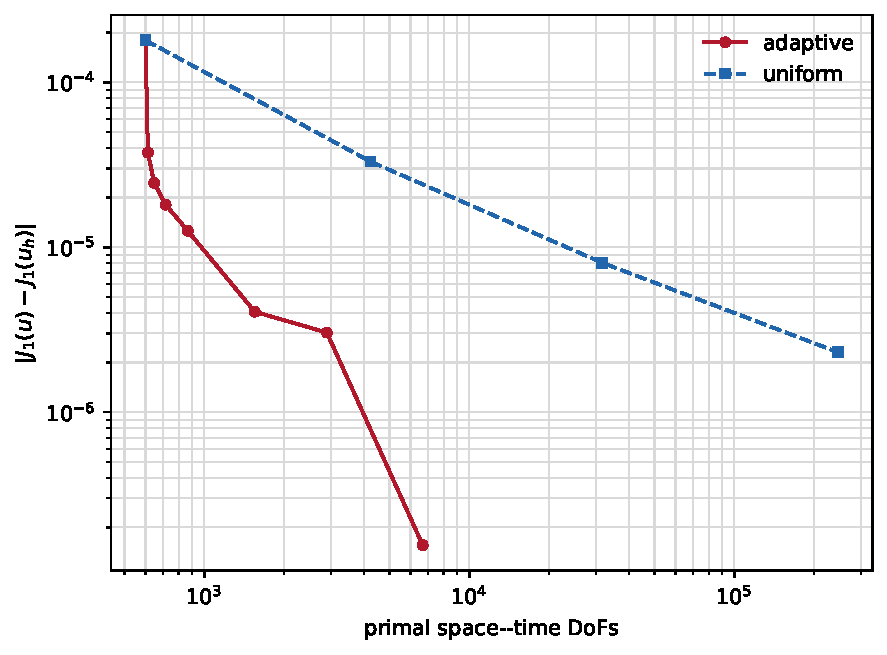
\includegraphics[width=0.65\textwidth]
    {figures/lshape/lshape_j1_adaptive_uniform.pdf}
  \caption{$J_1$ error against total primal space--time degrees of freedom for adaptive iterations 0--7 and the uniform sequence 0--3.}
  \label{fig:lshape-j1-comparison}
\end{figure}
\begin{table}[h]
  \centering
  \caption{Representative fitted-$J_1$ results.}
  \label{tab:lshape-j1-results}
  \small
  \setlength{\tabcolsep}{4pt}
  \begin{tabular}{lrrrrr}
    \toprule
    strategy/iterate & $N_{\mathrm{st}}$ & $N_t$ & $|e_{J_1}|$ & $I_{\mathrm{eff}}^{\mathrm{glob}}$ & $I_{\mathrm{eff}}^{\mathrm{loc}}$ \\
    \midrule
    initial           & $600$     & $8$  & $1.798\times10^{-4}$ & $0.925$ & $0.926$ \\
    uniform 1         & $4\,240$   & $16$ & $3.304\times10^{-5}$ & $1.082$ & $1.063$ \\
    uniform 2         & $31\,776$  & $32$ & $8.036\times10^{-6}$ & $1.023$ & $1.004$ \\
    uniform 3         & $245\,824$ & $64$ & $2.307\times10^{-6}$ & $1.007$ & $0.983$ \\
    % adaptive 1        & $613$      & $8$  & $3.748\times10^{-5}$ & $1.100$ & $1.074$ \\
    adaptive 2        & $647$      & $8$  & $2.450\times10^{-5}$ & $1.140$ & $1.106$ \\
    % adaptive 3        & $715$      & $8$  & $1.808\times10^{-5}$ & $1.194$ & $1.149$ \\
    adaptive 4        & $867$      & $8$  & $1.256\times10^{-5}$ & $1.062$ & $0.972$ \\
    adaptive 5        & $1\,551$   & $9$  & $4.060\times10^{-6}$ & $1.321$ & $1.092$ \\
    adaptive 6        & $2\,901$   & $11$ & $3.036\times10^{-6}$ & $0.970$ & $0.645$ \\
    adaptive 7        & $6\,673$  & $14$ & $1.561\times10^{-7}$ & $0.550$ & $4.358$ \\
    \bottomrule
  \end{tabular}
\end{table}

Thus uniform refinement uses approximately $245824/2901\simeq84.7$ times as many primal space--time degrees of freedom to reach a comparable goal accuracy. 
At the initial level the global and localised estimates are $-1.6628\times10^{-4}$ and $-1.6645\times10^{-4}$, giving effectivities $0.925$ and $0.926$, respectively. Uniform refinement subsequently drives both indices smoothly towards one. The adaptive global index remains between $0.925$ and $1.321$ through iterate~6, despite changing only a small fraction of the space--time cells.
An unexpected decrease to $I_{\mathrm{eff}}^{\mathrm{glob}}=0.550$ occurs at adaptive iterate~7. The available exact goal value shows that this is associated with a failure of the saturation property underlying the DWR reliability and efficiency theory \cite{ENDTMAYER202419}. With $u_h^+$ denoting the enriched primal solution, the observed ratio 
\begin{equation*}
  b_h^{\mathrm{obs}}
  :=\frac{|J_1(u)-J_1(u_h^+)|}{|J_1(u)-J_1(u_h)|}
  \label{eq:lshape-observed-saturation}
\end{equation*}
equals $0.1296<1$ at iterate~6, where the enriched approximation is clearly more accurate, but increases to $1.382>1$ at iterate~7. At the latter level the low-order goal error has crossed zero and has the very small magnitude $1.561\times10^{-7}$, whereas the enriched goal lies on the opposite side of the exact value with error $2.157\times10^{-7}$. Enrichment no longer reduces the goal error, and the saturation-based estimate is not guaranteed.

(how to address this, or is it a problem? though Ieff is incorrect but the error is indeed decreasing)
% If further accuracy is required, the enriched problem should be strengthened, for example by increasing its spatial or temporal polynomial degree.


Finally, Figure~\ref{fig:lshape-j1-meshes} and~\ref{fig:lshape-j1-3d} show the actual two-dimensional mesh carried by the selected time slab. 
\begin{figure}[h]
  \centering
  \begin{subfigure}[t]{0.31\textwidth}
    \centering
    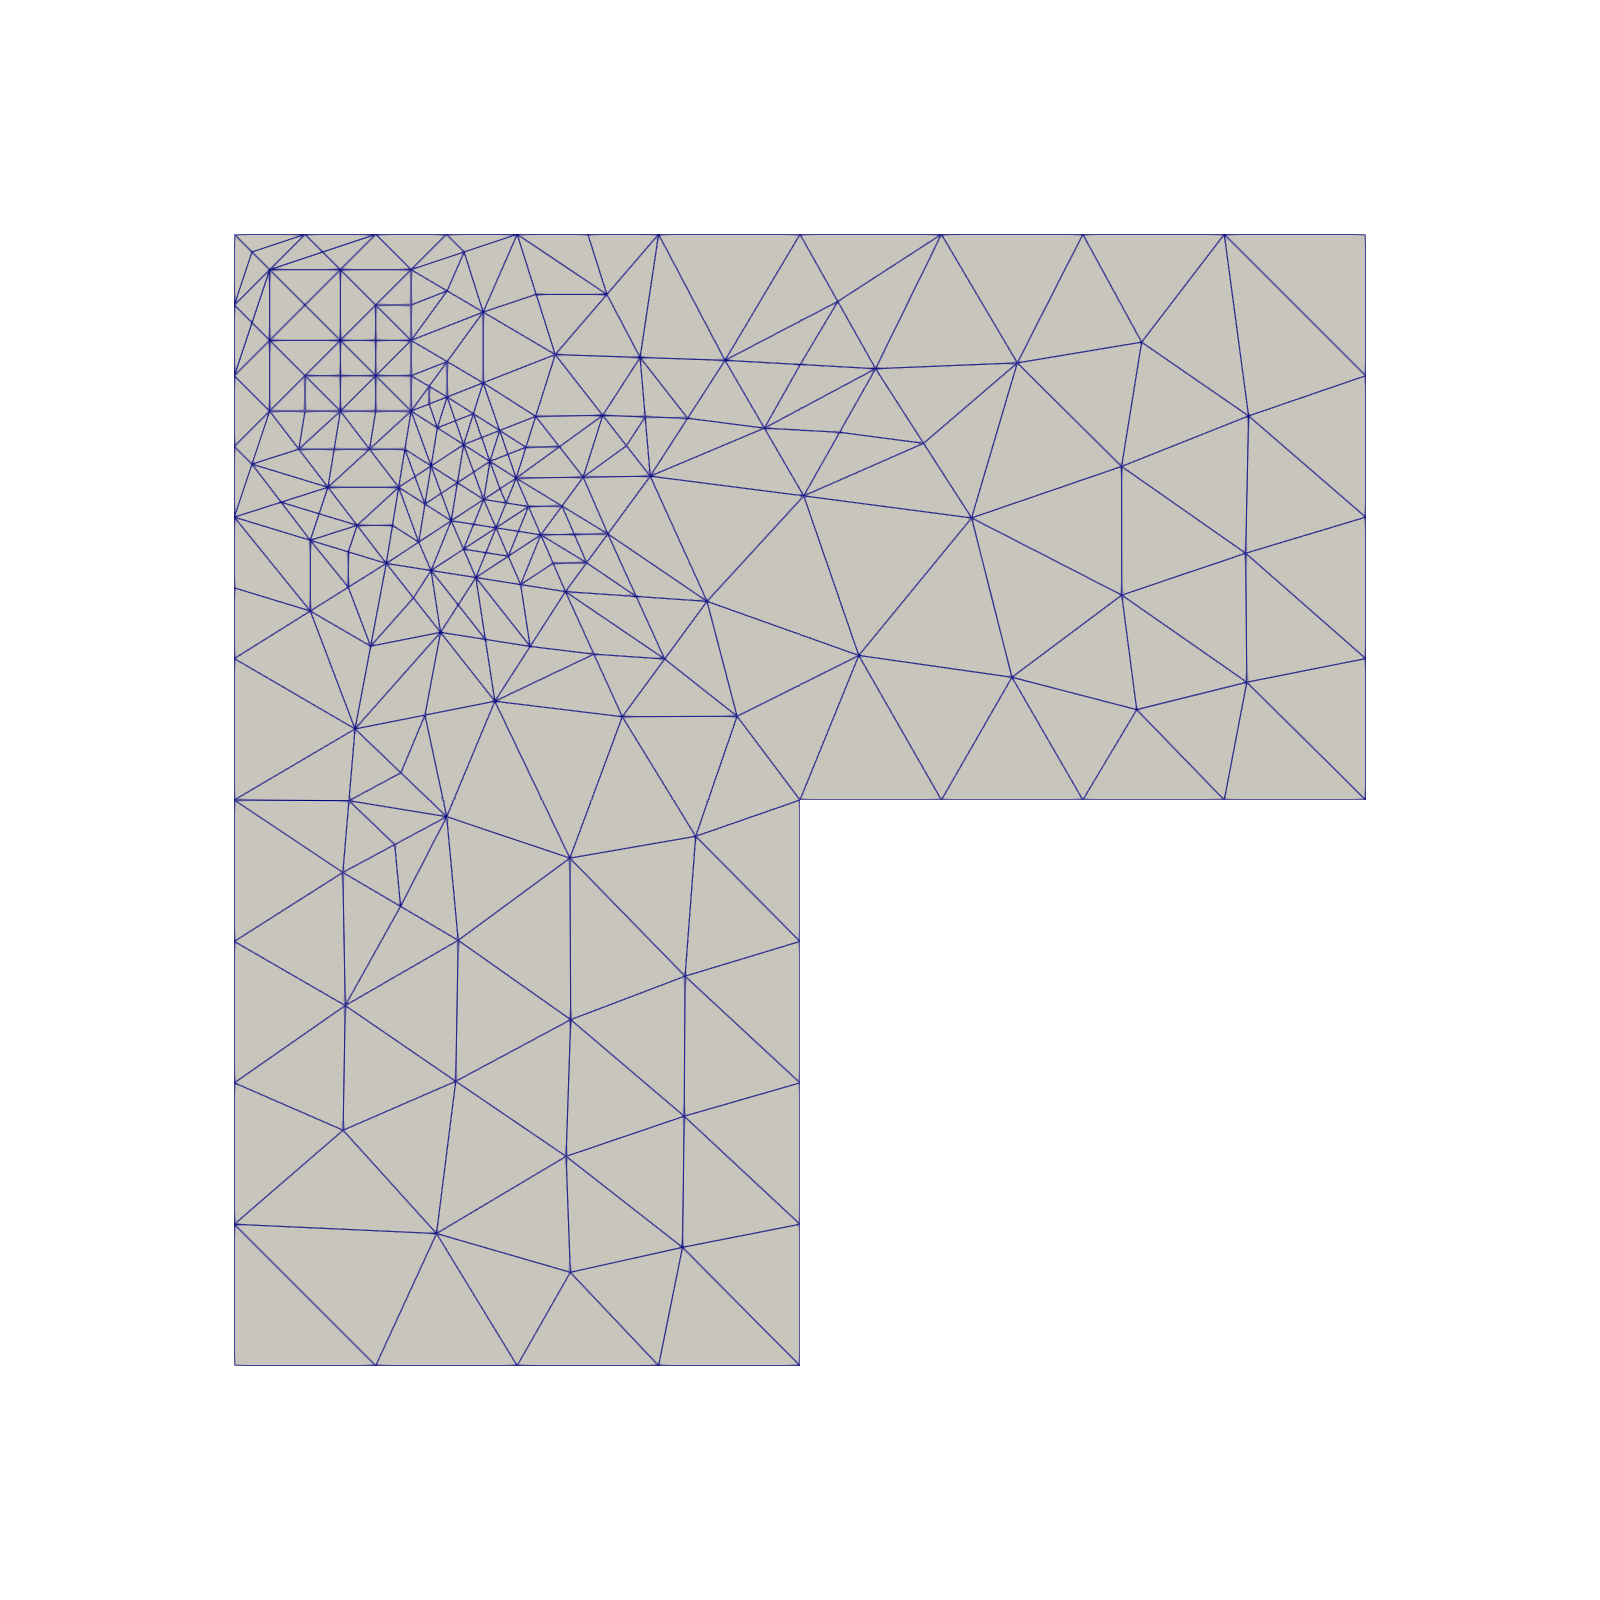
\includegraphics[
      width=\linewidth]{figures/lshape/j1_mesh.0000.png}
    \caption{}
  \end{subfigure}
  % \hfill
  \begin{subfigure}[t]{0.31\textwidth}
    \centering
    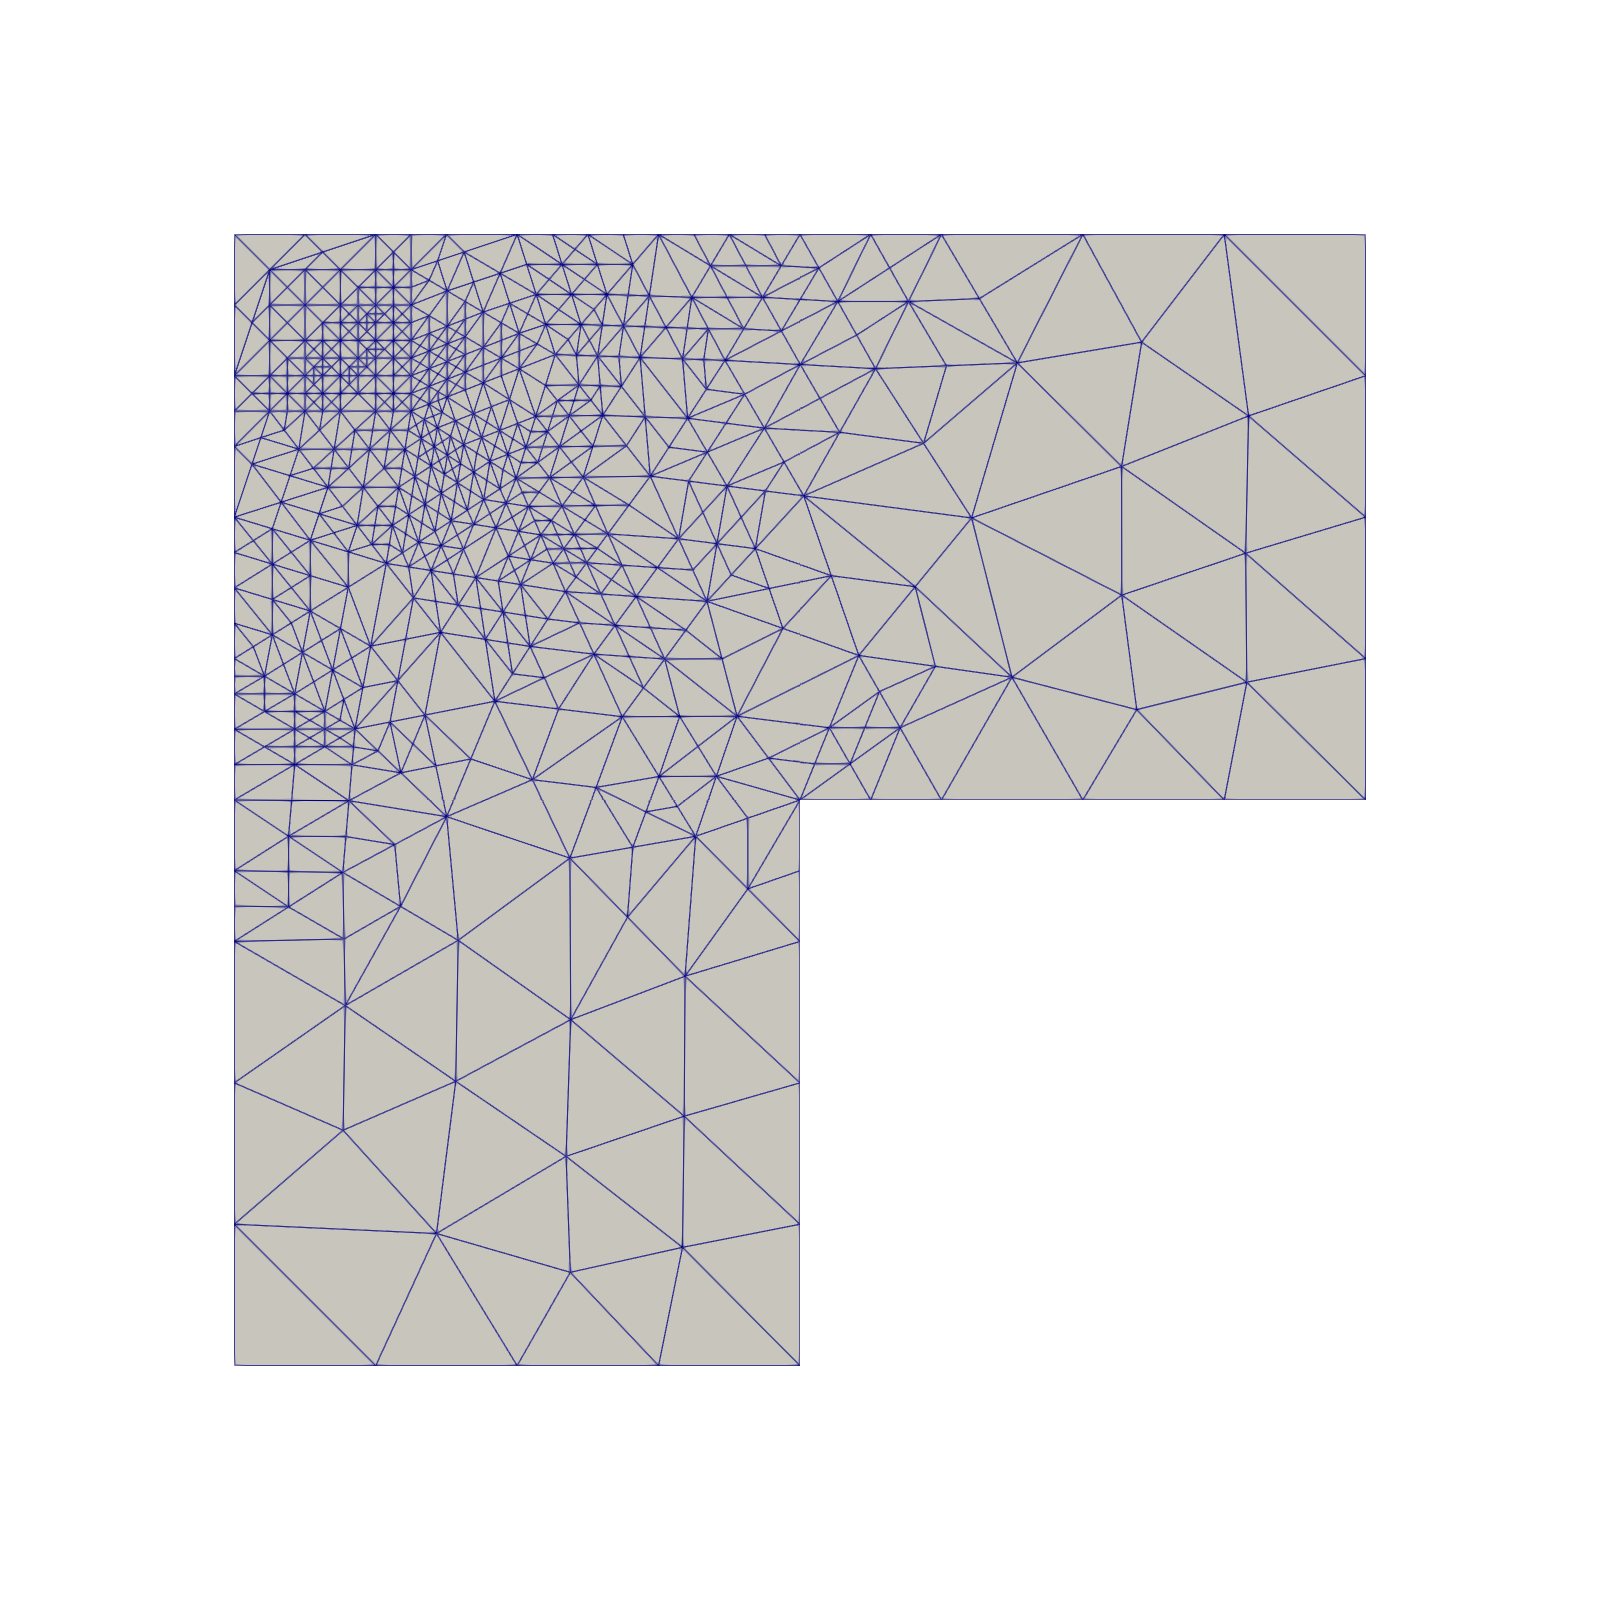
\includegraphics[
      width=\linewidth
    ]{figures/lshape/j1_mesh.0001.png}
    \caption{}
  \end{subfigure}
  \newline
  % \hfill
  \begin{subfigure}[t]{0.31\textwidth}
    \centering
    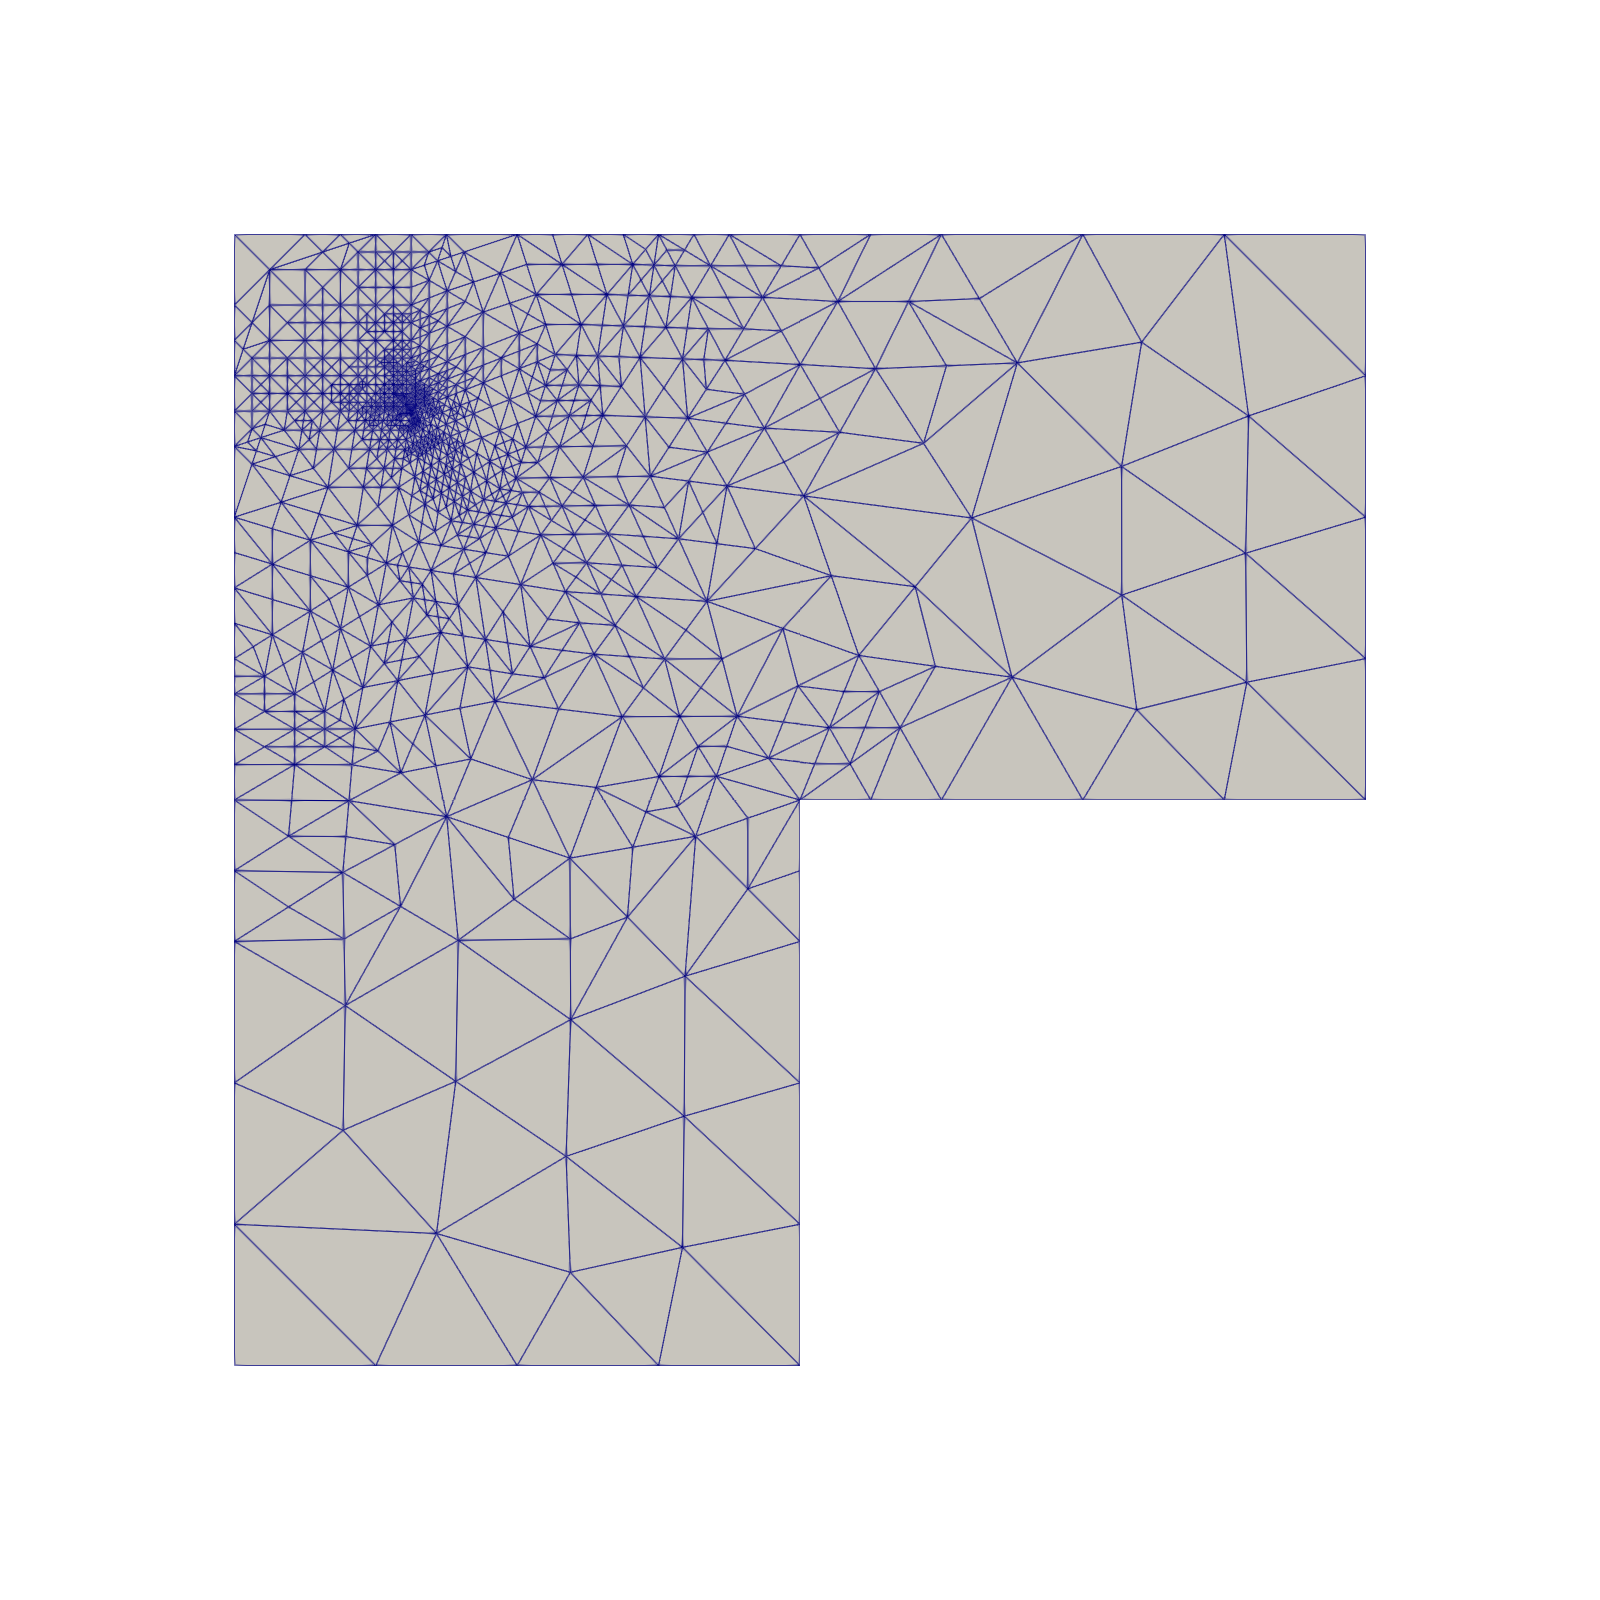
\includegraphics[
      width=\linewidth
    ]{figures/lshape/j1_mesh.0002.png}
    \caption{}
  \end{subfigure}
  \hfill
  \begin{subfigure}[t]{0.31\textwidth}
    \centering
    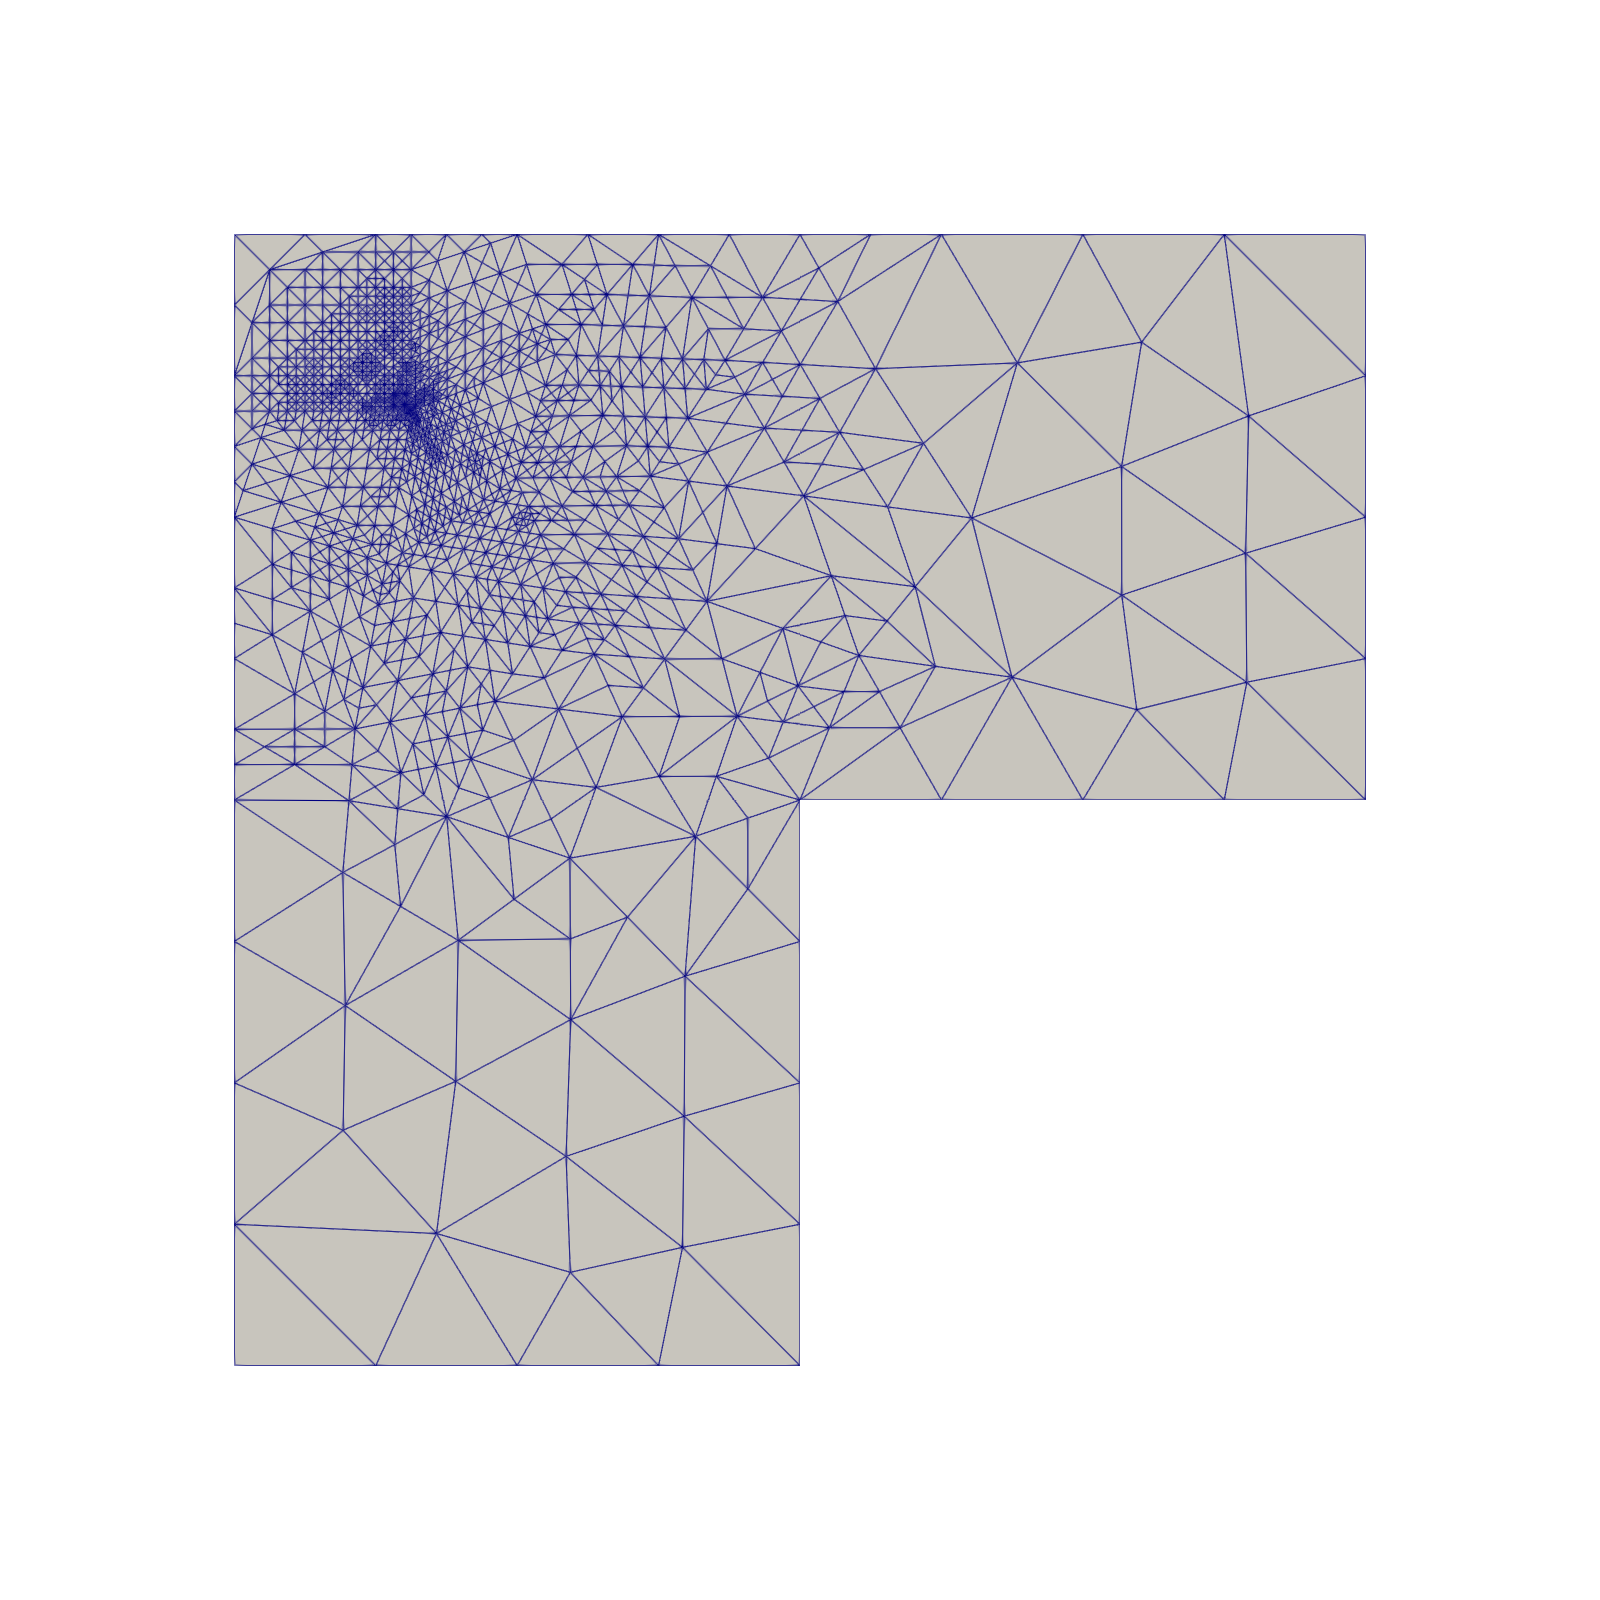
\includegraphics[
      width=\linewidth]{figures/lshape/j1_mesh.0003.png}
    \caption{}
  \end{subfigure}
  \hfill
  \begin{subfigure}[t]{0.31\textwidth}
    \centering
    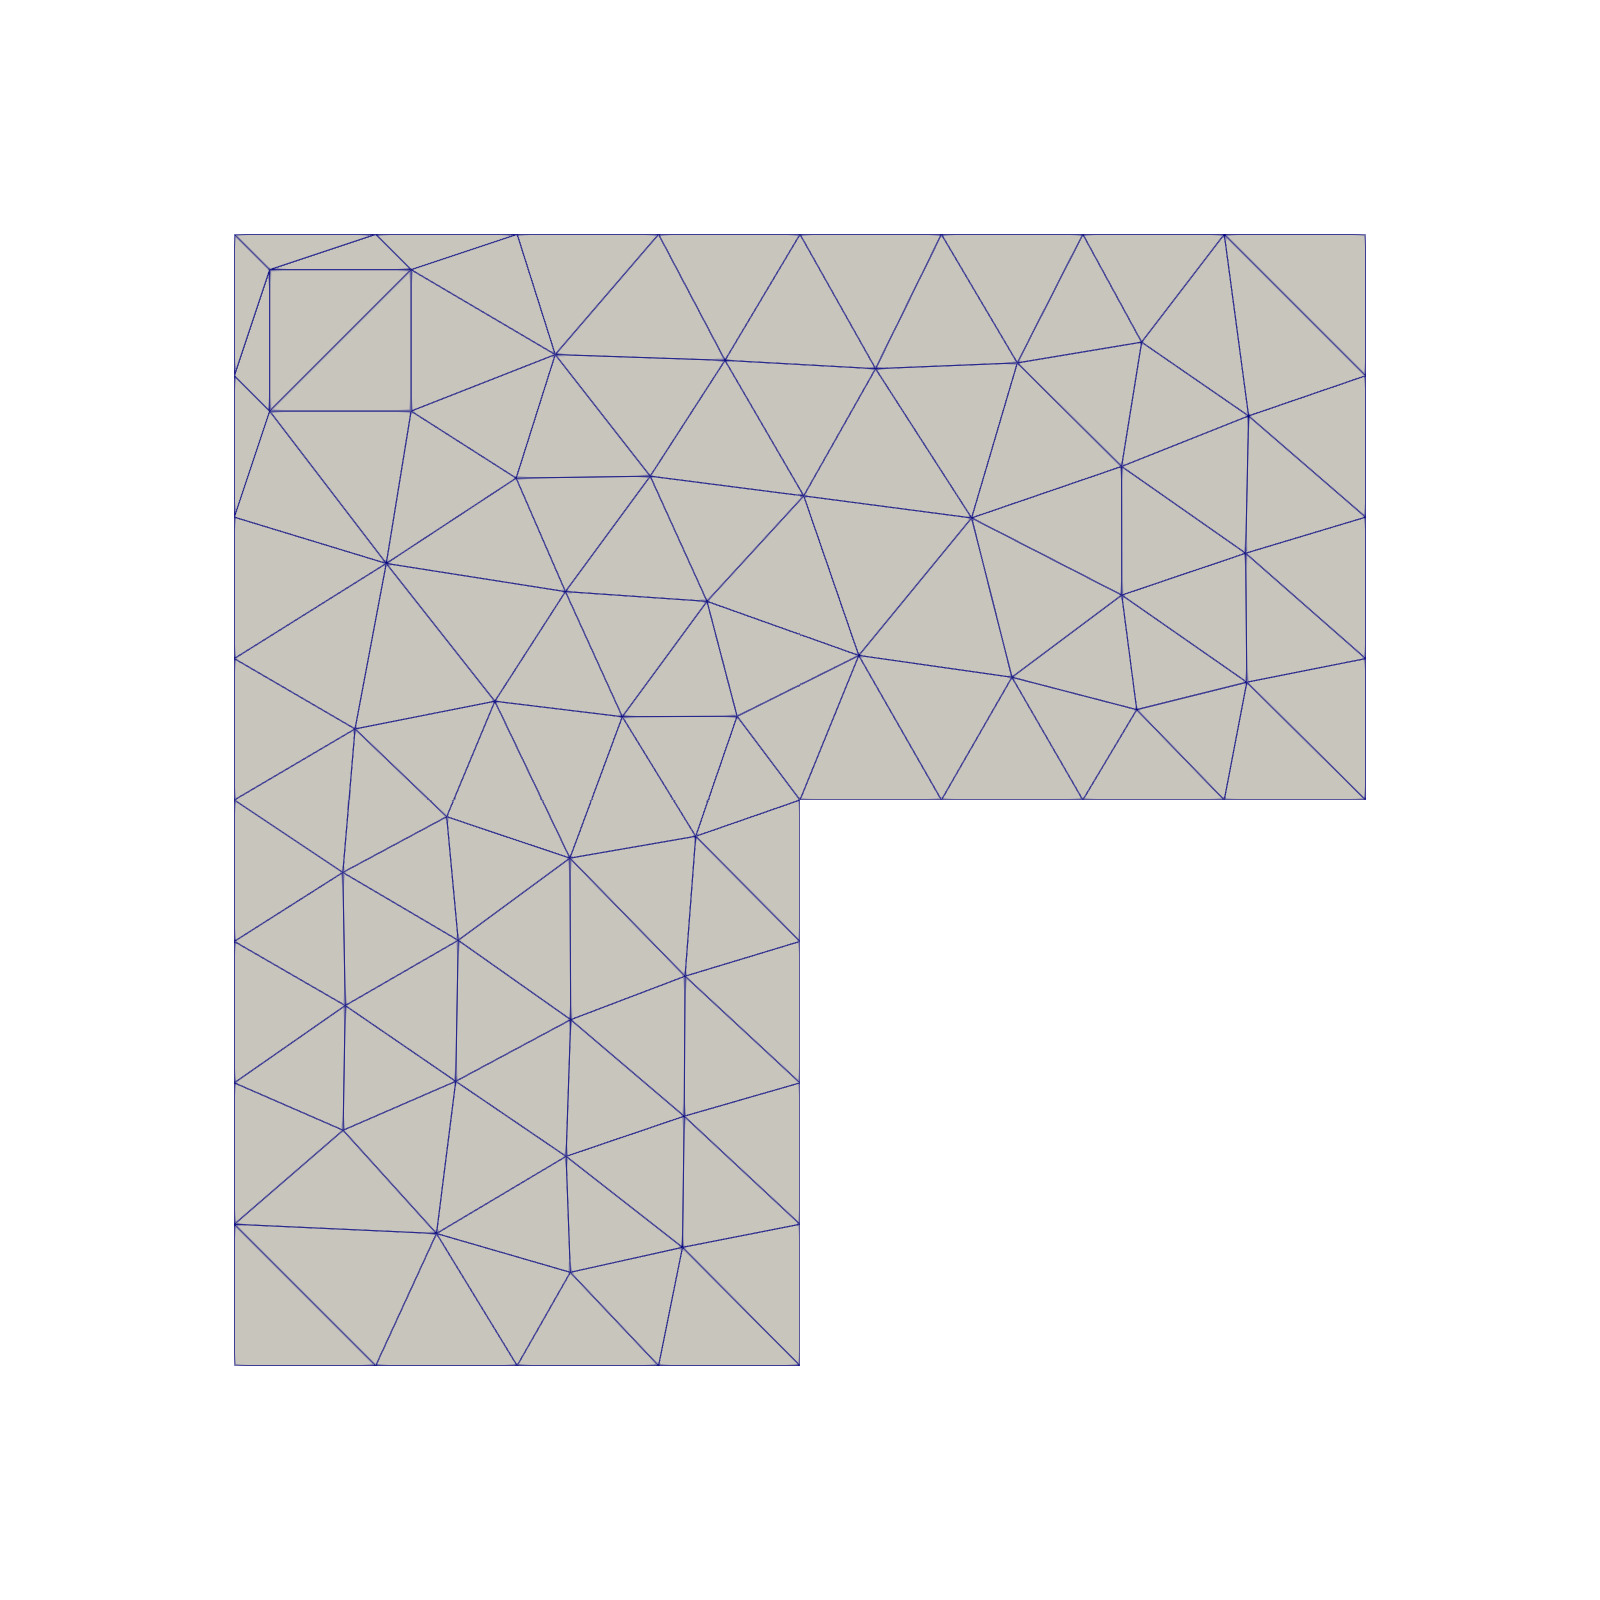
\includegraphics[
      width=\linewidth
    ]{figures/lshape/j1_mesh.0015.png}
    \caption{}
  \end{subfigure}
  \caption{Evolution of the slabwise spatial meshes. (a) shows the initial mesh, (b)--(e) show the spatial meshes carried by the adaptive time slabs whose right endpoints are $t=0.5$, $0.625$, $0.75$, and $1$, respectively.}
  \label{fig:lshape-j1-meshes}
\end{figure}
\begin{figure}[h]
  \centering
  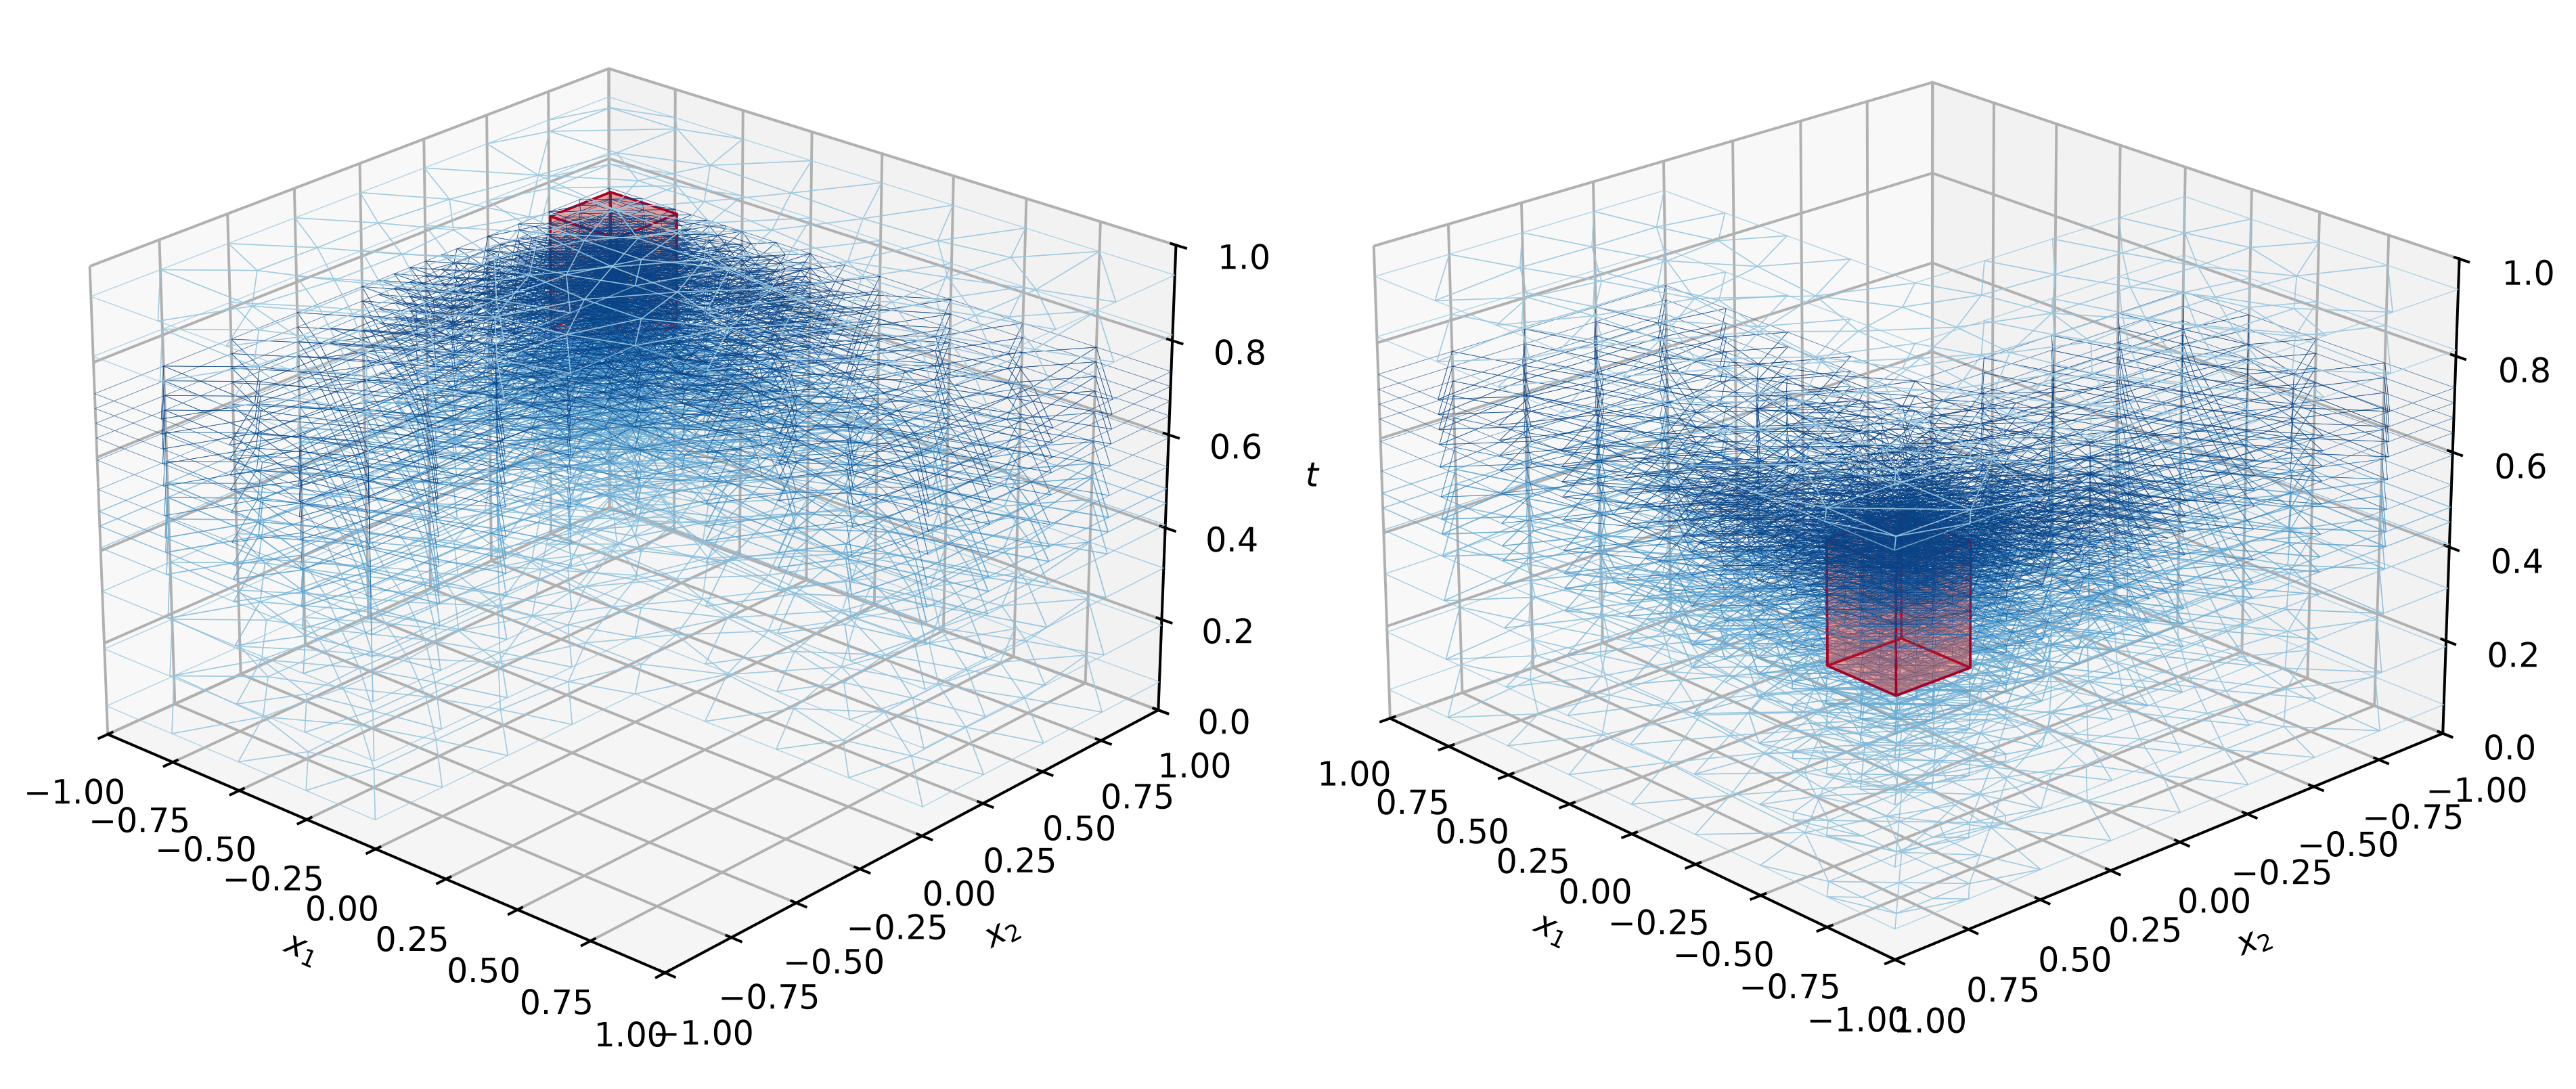
\includegraphics[width=0.95\textwidth]
    {figures/lshape/lshape_j1_spacetime_3d.png}
  \caption{Stacked representation of the slabwise spatial meshes at adaptive iterate~7, in exterior view and a view through the re-entrant corner, respectively. The red prism represents the space--time observation region $Q_I=\Omega_I\times[0.5,0.75]$.}
  \label{fig:lshape-j1-3d}
\end{figure}

The mesh sequence clarifies the source of the adaptive advantage. At $t=0.625$ the selected slab contains $1\,473$ cells and at $t=0.75$ it contains $1\,959$, whereas the terminal slab contains only the initial $116$ cells. Refinement is concentrated around $\Omega_I$ and its surrounding sensitivity region. It is not comparably dense at the re-entrant corner. This is consistent with the interpretation in \cite{ENDTMAYER202419}: the observation region is remote from the singularity. It is the DWR algorithm that does not attempt to resolve every loss of primal regularity. A norm-oriented estimator would be expected to prioritise the corner more strongly.

In summary, the L-shaped problem supplies the adaptive--uniform comparison that the preceding smooth tests did not stress. Here DWR-driven space-time adaptivity is more efficient than uniform refinement for the prescribed localised goal functional \(J_1\).


